% !TEX root = ../final-main.tex
\chapter{Enhancement-Mode Iteration 1}
\label{ch:iteration-1}

\section{Iteration 1 Process Plan}

Iteration 1 represented the first full device-level implementation of the
gate-recess process developed in Chapter~\ref{ch:gate-recess-process}. The
objective was to introduce a controlled recess beneath the Schottky gate while
retaining the established mesa isolation, ohmic contact formation, and gate
metallisation process used for the baseline depletion-mode devices.

\vspace{1mm}

The two enhancement-mode samples were initially processed together through the
common fabrication stages of mesa definition and ohmic contact formation (Figure~\ref{fig:mesa-liftoff}). 
This ensured that all quadrants shared an identical starting structure prior to the
recess and gate formation stages.

\vspace{1mm}

To use cleanroom time efficiently, two quadrants across the two samples were
processed in parallel. Completing the full device set across eight quadrants
therefore required four repeated cycles of recess lithography, recess etching,
gate lithography, and gate deposition.

\vspace{2mm}
\begin{figure}[htbp]
  \centering
  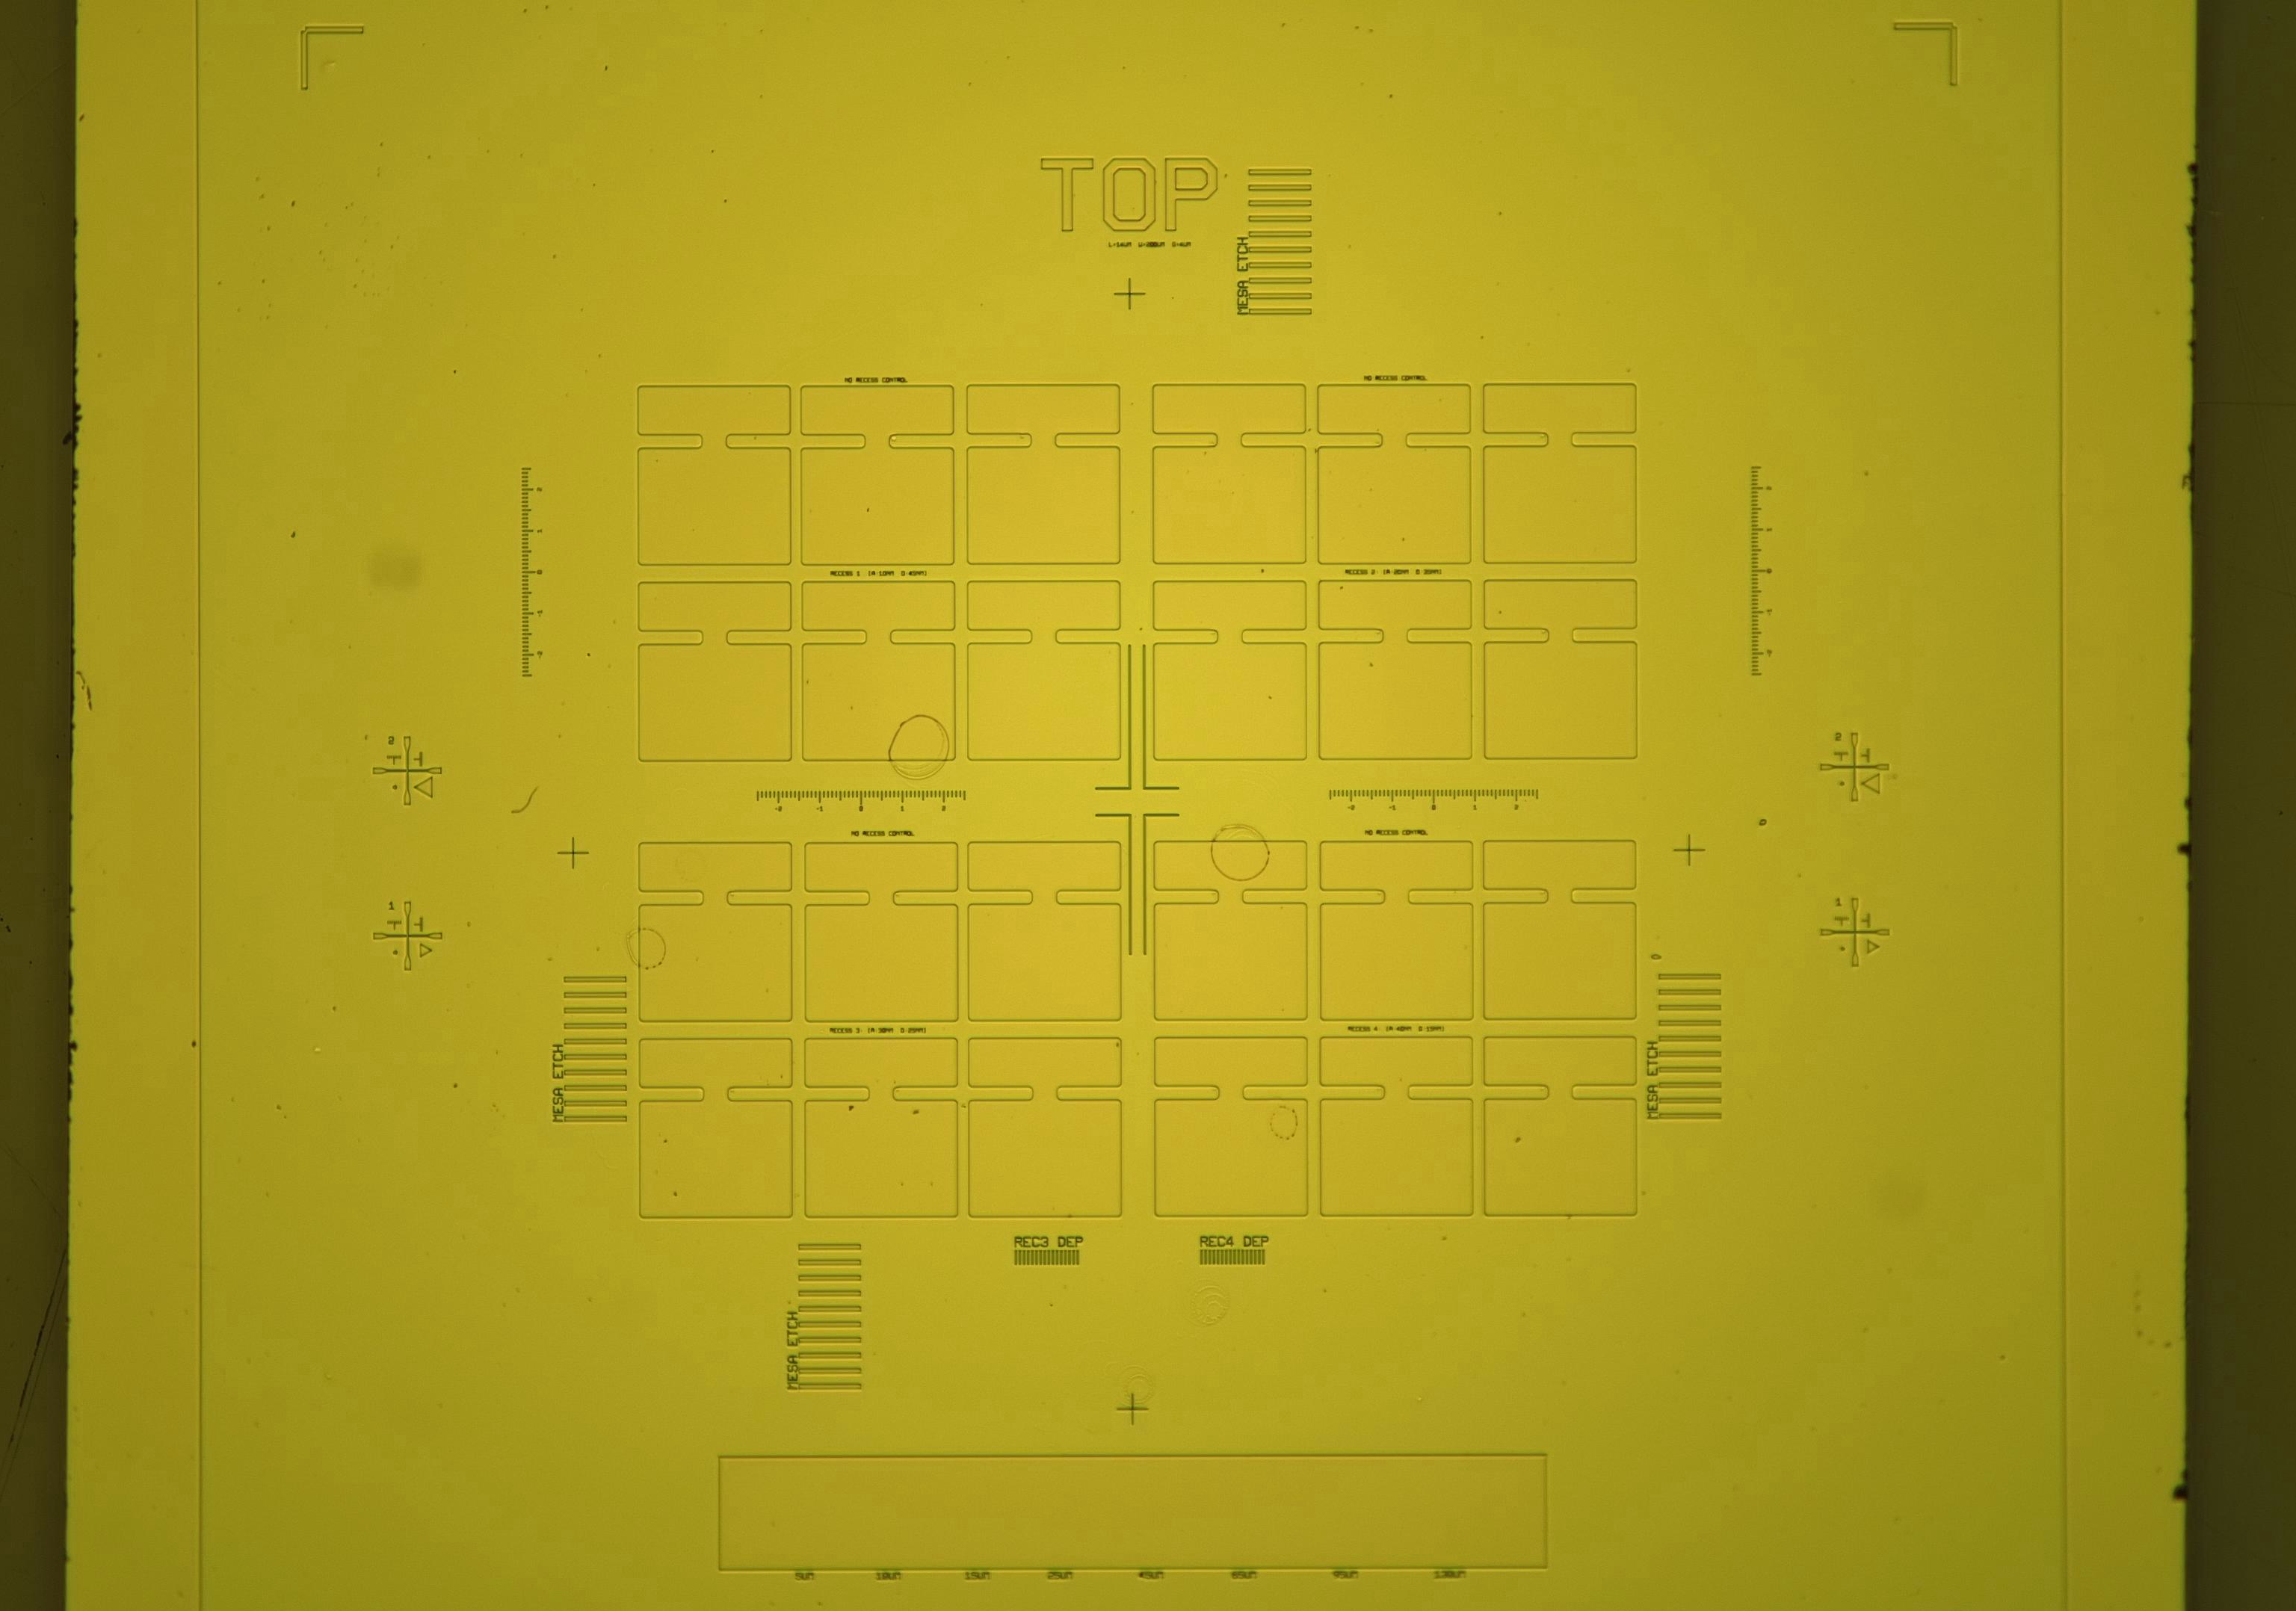
\includegraphics[width=0.48\linewidth]{figures/fabrication_images/enhancement_mode_images/mesa_etch_2-cropped.jpg}
  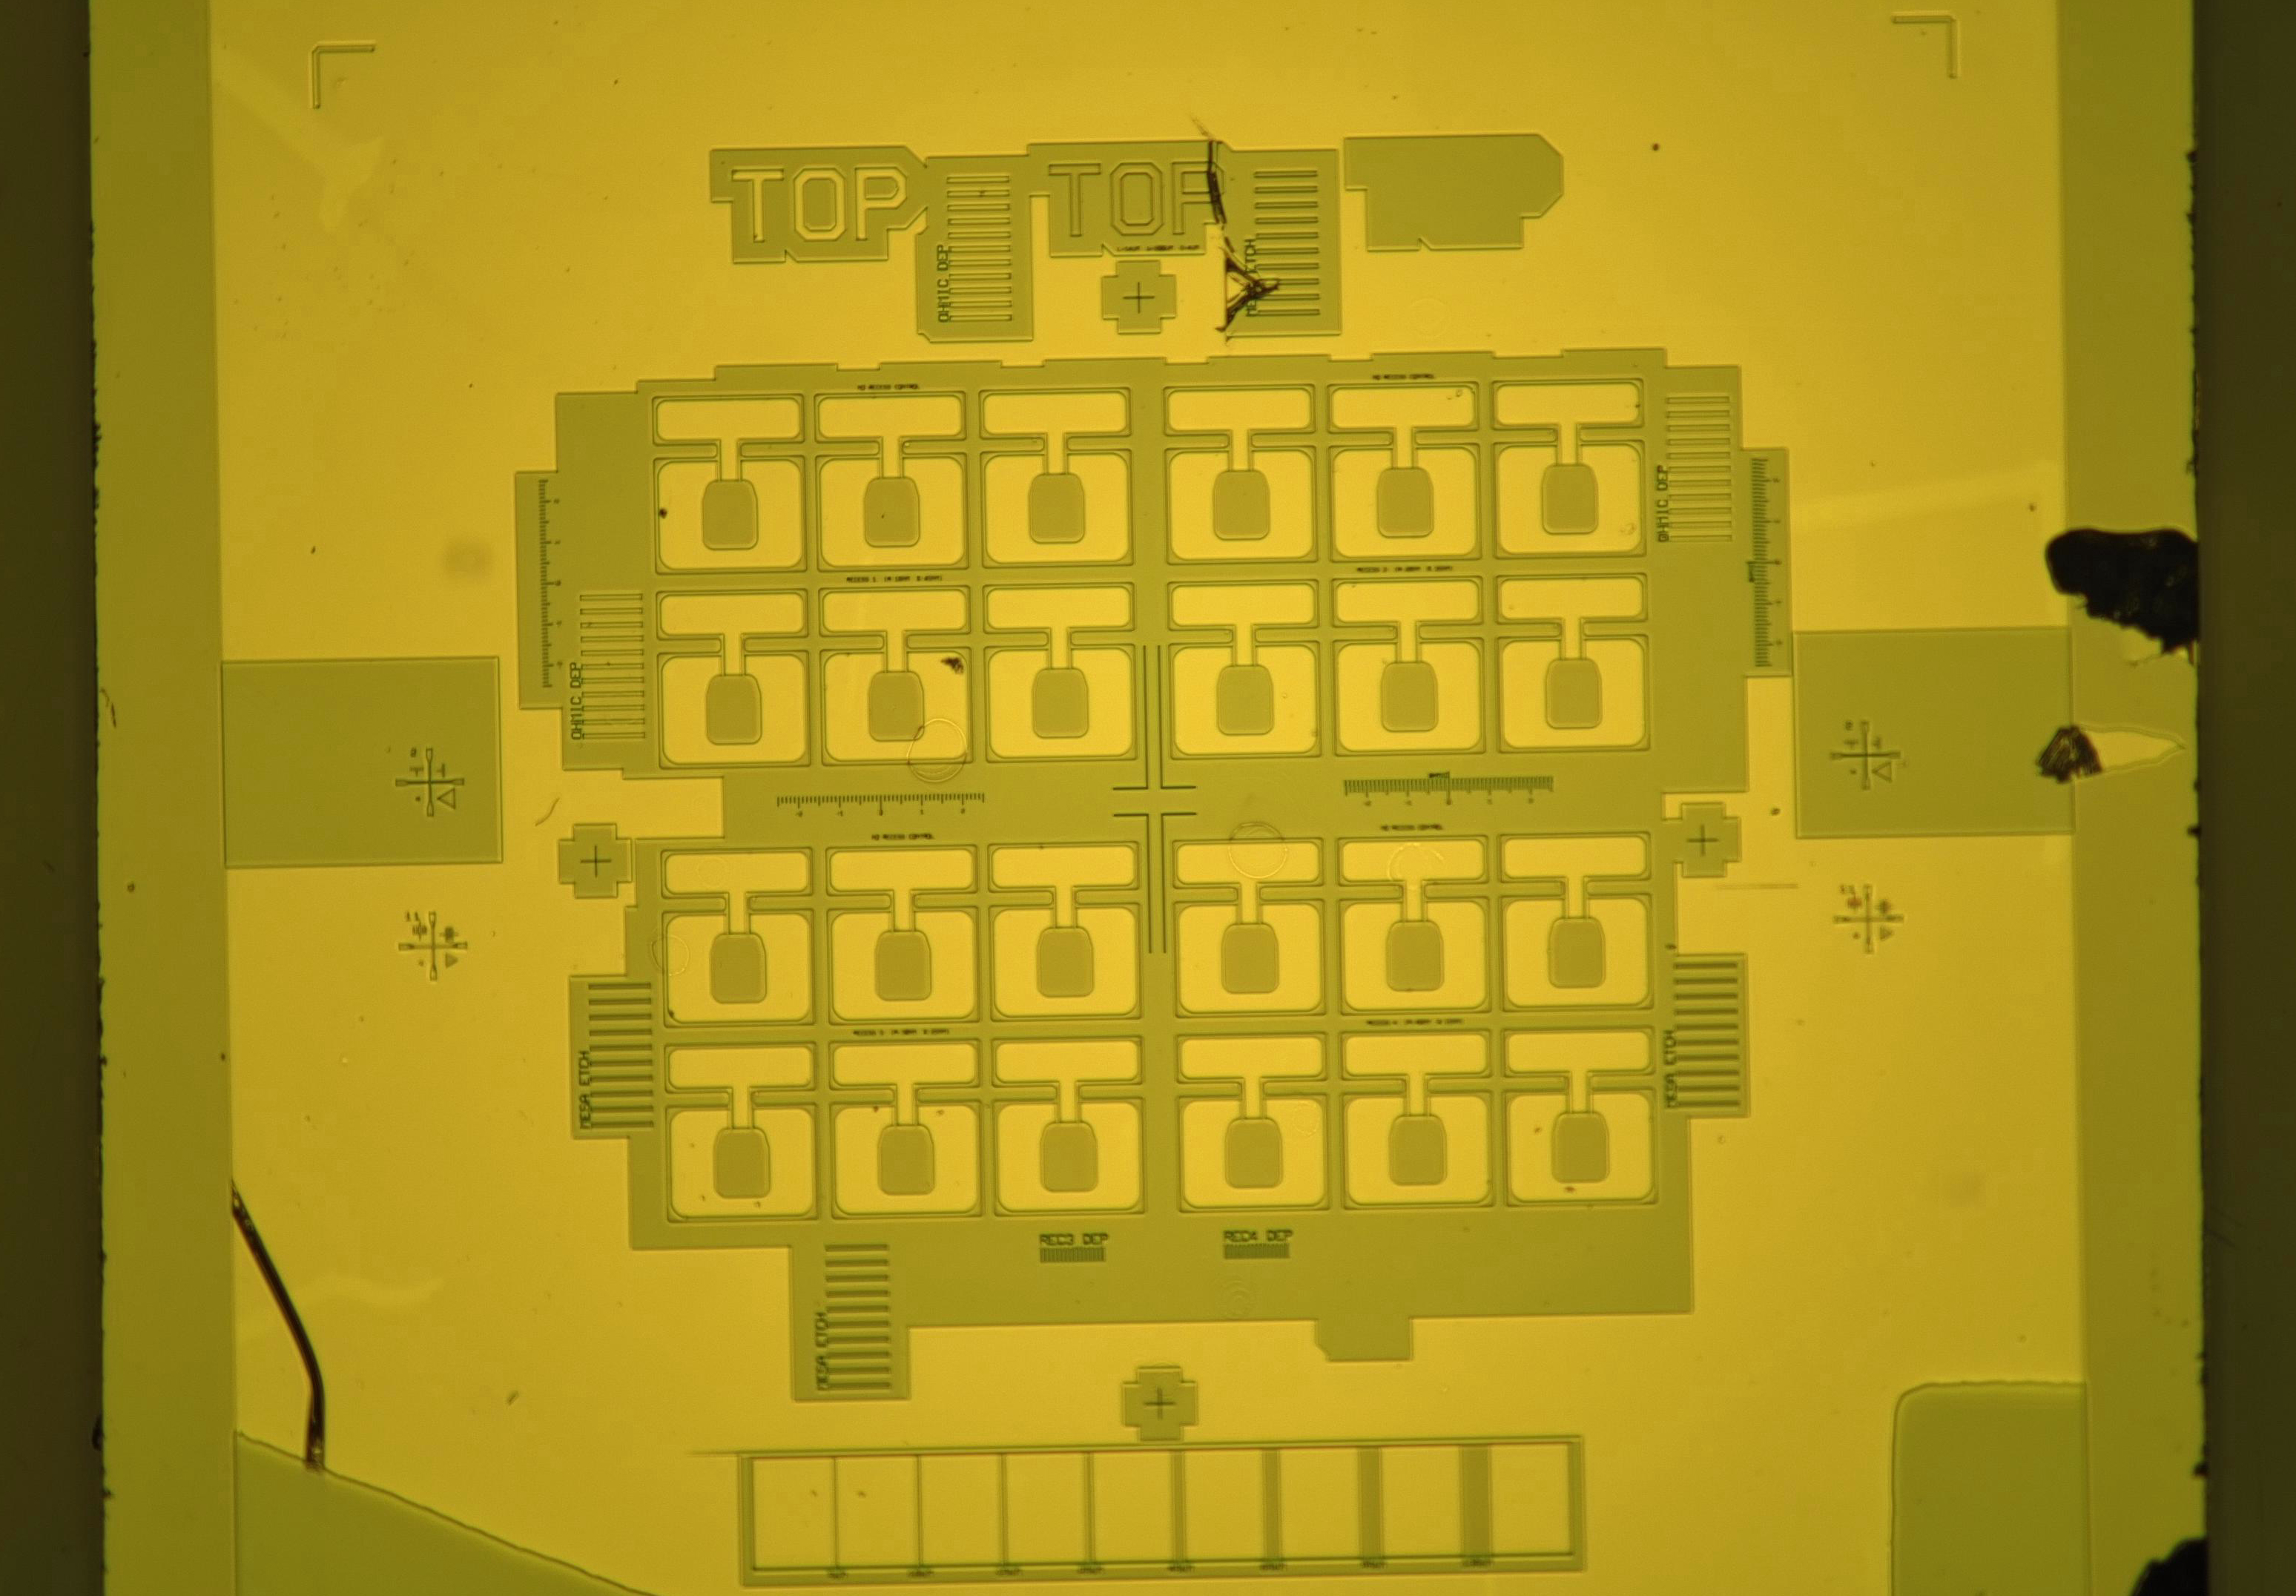
\includegraphics[width=0.48\linewidth]{figures/fabrication_images/enhancement_mode_images/ohmic_liftoff_2-cropped.jpg}
  \vspace{3pt}
  \caption{Mesa Formation and Ohmic Contact Development for the Enhancement
  Mode Device Set}
  \label{fig:mesa-liftoff}
\end{figure}

Each quadrant pair therefore represented an independent fabrication run,
including its own recess etch, gate formation process, and subsequent
electrical characterisation. Each quadrant pair
required approximately two days of processing. Consequently, variation between
quadrant pairs may reflect not only the intended recess-depth differences, but
also small run-to-run process variations introduced during the repeated
fabrication sequence.

\vspace{1mm}

This chapter focuses on the two device sets from the first
iteration of recessed devices. These were designed with nominal recess targets
of \SI{25}{\nano\metre} and \SI{30}{\nano\metre}, chosen to lie close to and
above the theoretical threshold depth derived in
Section~\ref{sec:threshold-voltage}. If the recess process behaved as intended,
these devices were expected to show a substantial positive shift in threshold
voltage relative to the unrecessed depletion mode devices.

\vspace{2mm}

\section{Mask Geometry and Intended Operation}

The Iteration 1 mask introduced the gate recess etch as two narrow slit
openings positioned between the source and drain contacts. These slits were
placed along the direct path between source and drain, so that the
material beneath the intended gate region could be locally recessed while
leaving the surrounding HEMT structure unchanged.

\vspace{1mm}

As discussed previously, the gate mask was deliberately designed to be wider 
than the recess etch mask, extending the mask by \SI{0.5}{\micro\metre} 
beyond the recess opening on either side. 
This overlap was included for the reason discussed in
Chapter~\ref{ch:gate-recess-process}: the gate metal must cover the etched
trench rather than sitting only on the original semiconductor surface. By
making the gate wider than the recess slit, the process allowed for alignment
tolerance between the recess lithography and the gate lithography while still
ensuring that the gate covered the recessed region.

\vspace{4mm}

% ------------------------------------------------------------
% File: figures/fig-iteration-1-mask-popout.tex
% Iteration 1 mask callout: device mask -> gate mask -> dimensions
% ------------------------------------------------------------

\begin{figure}[htbp]
  \centering
  \begin{tikzpicture}[
    font=\footnotesize,
    callout/.style={dashed, line width=0.8pt},
    connector/.style={dashed, line width=0.45pt, opacity=0.45},
    imagebox/.style={draw, line width=0.4pt, inner sep=2pt},
    figlabel/.style={draw, fill=white, line width=0.35pt, inner xsep=4pt,
      inner ysep=2pt, font=\small\bfseries}
  ]
    % Manual adjustment controls:
    % - Device image size: change the width in the device \includegraphics.
    % - Red source box on device mask: change \devBoxLeft, \devBoxRight,
    %   \devBoxTop, and \devBoxBottom. These are fractions of the image width
    %   and height from the image edges.
    % - Red source box on the device mask: these are image fractions from
    %   the top-left of the device image. The current box is landscape and
    %   matches the physical aspect ratio of gate_mask.png.
    \def\devBoxLeft{0.305}
    \def\devBoxRight{0.685}
    \def\devBoxTop{0.250}
    \def\devBoxBottom{0.500}
    % - Blue source box on the gate mask: currently placed just right of
    %   centre height, over one recess region. Adjust these fractions after
    %   checking the compiled image.
    \def\gateBlueLeft{0.705}
    \def\gateBlueRight{0.845}
    \def\gateBlueTop{0.44}
    \def\gateBlueBottom{0.58}

    % Top-level device mask.
    \node[imagebox, anchor=north west] (device) at (0,0) {
      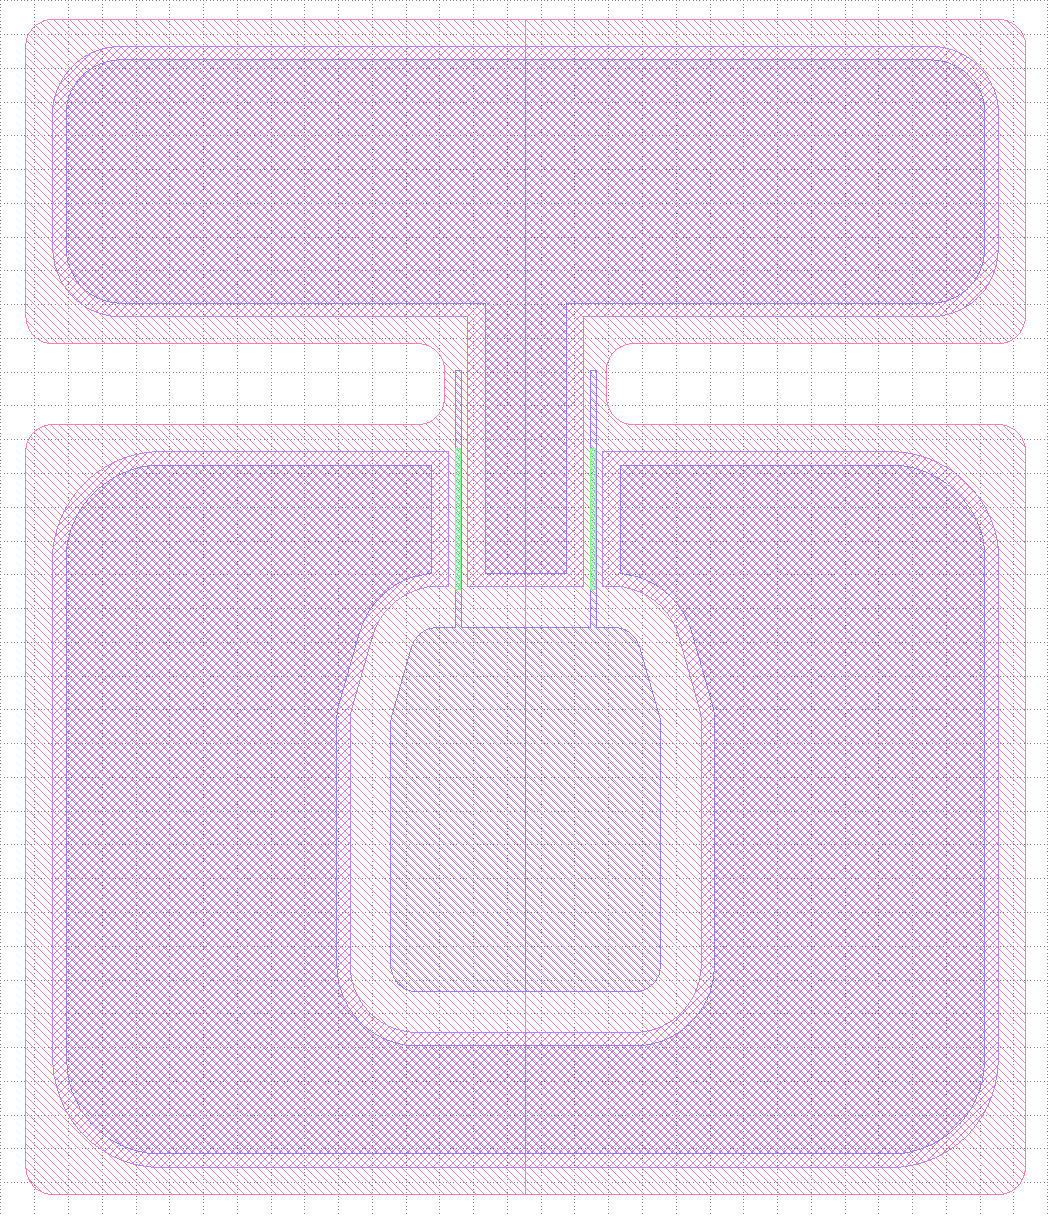
\includegraphics[width=0.28\linewidth]{figures/gate_recession/device_mask.png}
    };
    \node[figlabel, anchor=north, yshift=-1.5mm] (deviceLabel) at (device.south) {Single Device Mask};

    % Pop-out gate mask.
    \node[imagebox, anchor=north west] (gate) at (7.1,0) {
      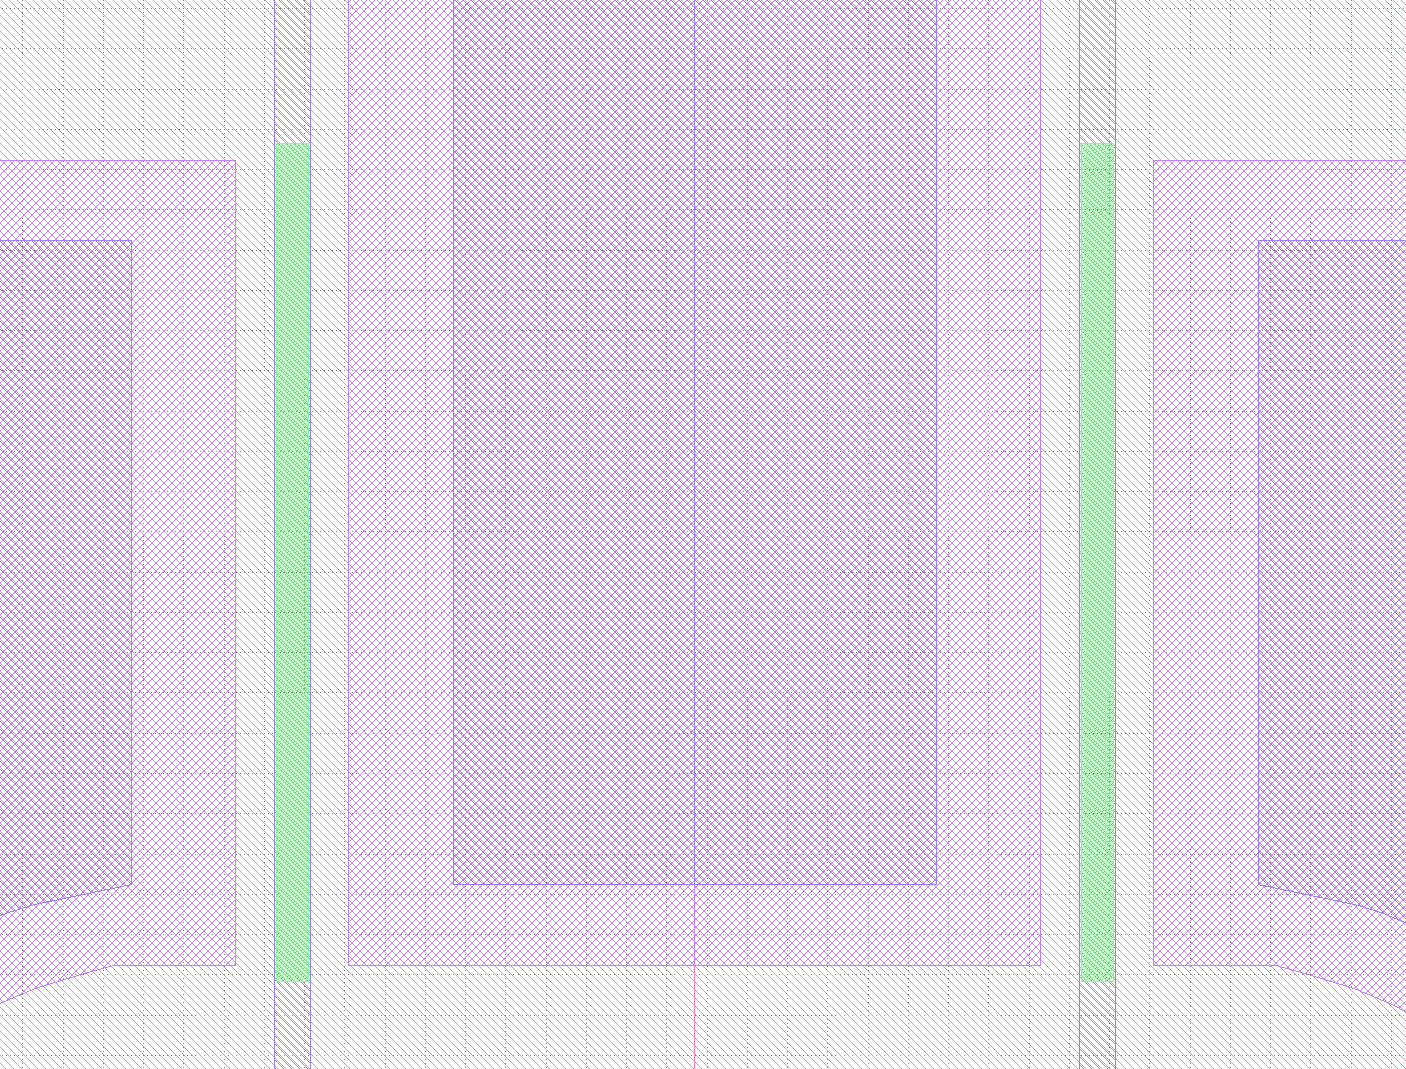
\includegraphics[width=0.426\linewidth]{figures/gate_recession/gate_mask.png}
    };
    \node[figlabel, anchor=north, yshift=-1.5mm] (gateLabel) at (gate.south) {Gate/Recess Mask Zoomed};

    % Lower dimensions pop-out.
    \node[imagebox, anchor=north] (dimensions) at ($(device.south west)!0.5!(gate.south east)+(0,-1.10)$) {
      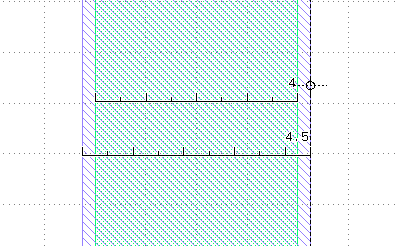
\includegraphics[width=0.64\linewidth]{figures/gate_recession/mask_dimensions.png}
    };
    \node[figlabel, anchor=north, yshift=-1.5mm] (dimensionsLabel) at (dimensions.south) {Gate/Recess Mask Dimensions};

    % Red source callout on the device mask.
    \path let \p1=(device.north west), \p2=(device.south east) in
      coordinate (deviceBoxNW) at ({\x1+\devBoxLeft*(\x2-\x1)}, {\y1+\devBoxTop*(\y2-\y1)})
      coordinate (deviceBoxNE) at ({\x1+\devBoxRight*(\x2-\x1)}, {\y1+\devBoxTop*(\y2-\y1)})
      coordinate (deviceBoxSW) at ({\x1+\devBoxLeft*(\x2-\x1)}, {\y1+\devBoxBottom*(\y2-\y1)})
      coordinate (deviceBoxSE) at ({\x1+\devBoxRight*(\x2-\x1)}, {\y1+\devBoxBottom*(\y2-\y1)});

    \draw[callout, red!75!black]
      (deviceBoxNW) rectangle (deviceBoxSE);

    % Pop-out target box on the gate mask. Currently surrounds the full image.
    \coordinate (gateRedNW) at ($(gate.north west)+(0.08,-0.08)$);
    \coordinate (gateRedNE) at ($(gate.north east)+(-0.08,-0.08)$);
    \coordinate (gateRedSW) at ($(gate.south west)+(0.08,0.08)$);
    \coordinate (gateRedSE) at ($(gate.south east)+(-0.08,0.08)$);
    \draw[callout, red!75!black]
      (gateRedNW) rectangle (gateRedSE);

    % Blue source callout on the gate mask.
    \path let \p1=(gate.north west), \p2=(gate.south east) in
      coordinate (gateBlueNW) at ({\x1+\gateBlueLeft*(\x2-\x1)}, {\y1+\gateBlueTop*(\y2-\y1)})
      coordinate (gateBlueNE) at ({\x1+\gateBlueRight*(\x2-\x1)}, {\y1+\gateBlueTop*(\y2-\y1)})
      coordinate (gateBlueSW) at ({\x1+\gateBlueLeft*(\x2-\x1)}, {\y1+\gateBlueBottom*(\y2-\y1)})
      coordinate (gateBlueSE) at ({\x1+\gateBlueRight*(\x2-\x1)}, {\y1+\gateBlueBottom*(\y2-\y1)});

    \draw[callout, blue!70!black]
      (gateBlueNW) rectangle (gateBlueSE);

    \coordinate (dimBlueNW) at ($(dimensions.north west)+(0.08,-0.08)$);
    \coordinate (dimBlueNE) at ($(dimensions.north east)+(-0.08,-0.08)$);
    \coordinate (dimBlueSW) at ($(dimensions.south west)+(0.08,0.08)$);
    \coordinate (dimBlueSE) at ($(dimensions.south east)+(-0.08,0.08)$);
    \draw[callout, blue!70!black]
      (dimBlueNW) rectangle (dimBlueSE);

    % Device mask -> gate mask pop-out connectors. These are drawn above the
    % device mask, then the gate/recess mask panel is redrawn over them.
    \draw[connector, red!75!black]
      (deviceBoxNW) --
      (gateRedNW);
    \draw[connector, red!75!black]
      (deviceBoxNE) --
      (gateRedNE);
    \draw[connector, red!75!black]
      (deviceBoxSW) --
      (gateRedSW);
    \draw[connector, red!75!black]
      (deviceBoxSE) --
      (gateRedSE);

    % Redraw the gate/recess mask panel so red connector lines sit beneath it.
    \node[imagebox, anchor=north west] at (gate.north west) {
      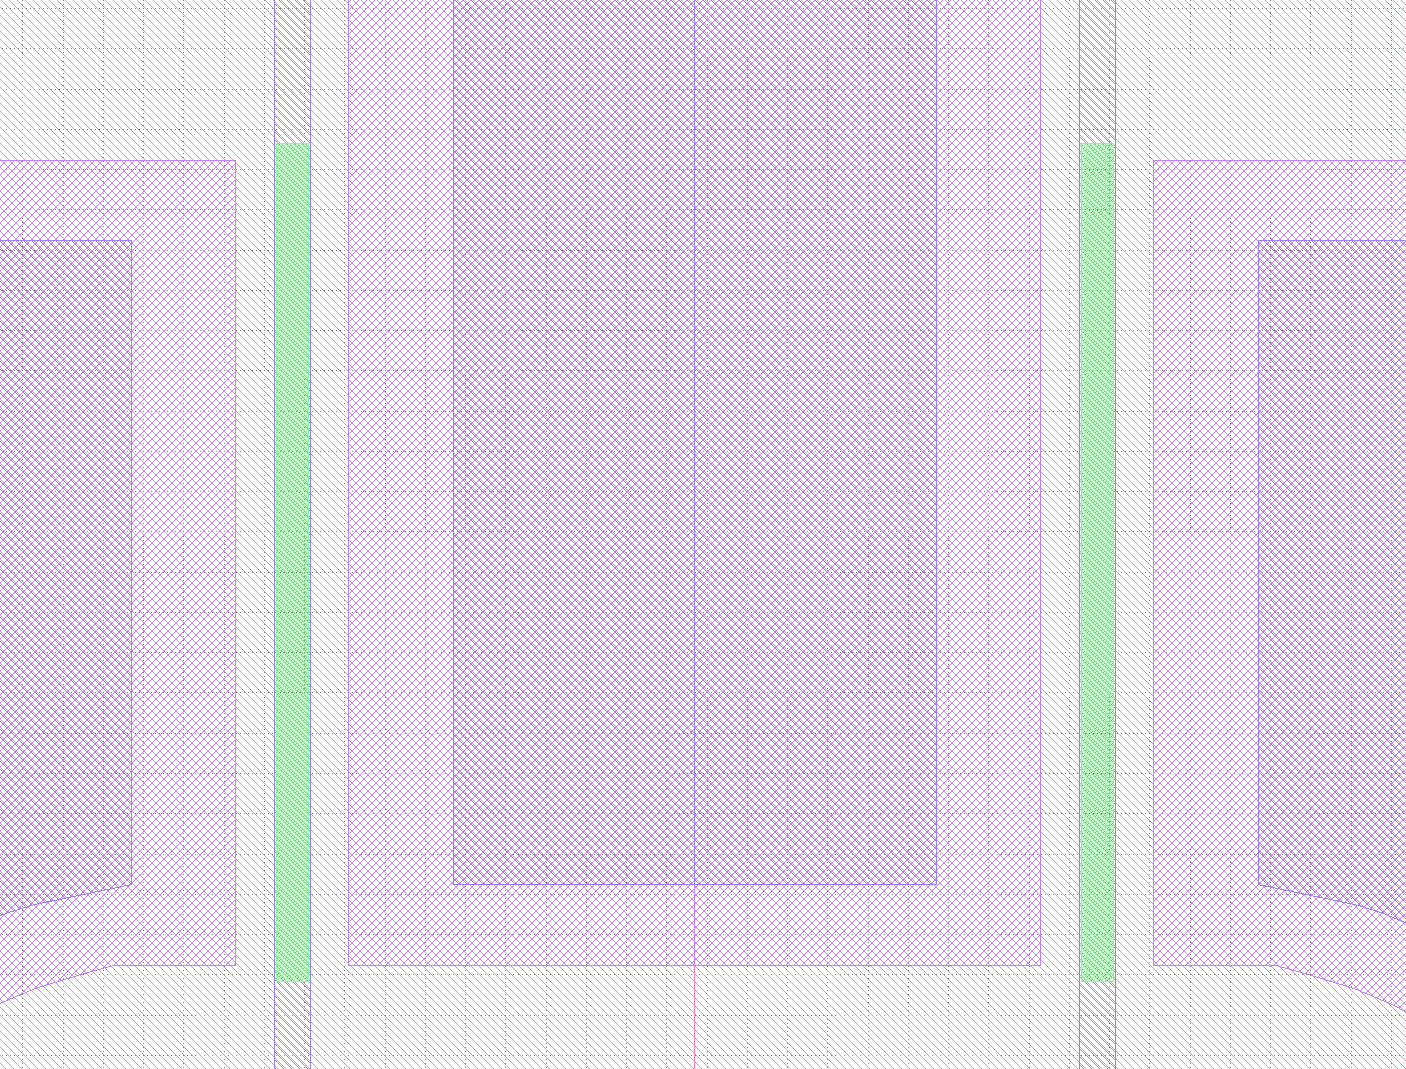
\includegraphics[width=0.426\linewidth]{figures/gate_recession/gate_mask.png}
    };
    \draw[callout, red!75!black]
      (gateRedNW) rectangle (gateRedSE);
    \draw[callout, blue!70!black]
      (gateBlueNW) rectangle (gateBlueSE);

    % Gate mask -> dimensions pop-out connectors. These are drawn above the
    % gate/recess mask, then the dimensions panel is redrawn over them.
    \draw[connector, blue!70!black]
      (gateBlueNW) --
      (dimBlueNW);
    \draw[connector, blue!70!black]
      (gateBlueNE) --
      (dimBlueNE);
    \draw[connector, blue!70!black]
      (gateBlueSW) --
      (dimBlueSW);
    \draw[connector, blue!70!black]
      (gateBlueSE) --
      (dimBlueSE);

    % Redraw the dimensions panel so blue connector lines sit beneath it.
    \node[imagebox, anchor=north] at (dimensions.north) {
      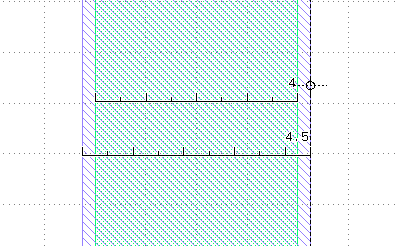
\includegraphics[width=0.64\linewidth]{figures/gate_recession/mask_dimensions.png}
    };
    \draw[callout, blue!70!black]
      (dimBlueNW) rectangle (dimBlueSE);

    % Redraw labels above connector lines.
    \node[figlabel, anchor=north, yshift=-1.5mm] at (device.south) {Single Device mask};
    \node[figlabel, anchor=north, yshift=-1.5mm] at (gate.south) {Gate/Recess Mask Zoomed};
    \node[figlabel, anchor=north, yshift=-1.5mm] at (dimensions.south) {Gate/Recess Mask Dimensions};
  \end{tikzpicture}

  \vspace{2mm}
  \caption{Iteration 1 mask structure with device-level, gate/recess, and
  dimensioned views.}
  \label{fig:iteration-1-mask}
\end{figure}


\vspace{1mm}

\section{Recess Etch Measurements}

After the recess etch, the etched depths were measured using the Alpha-Step
surface profiler. The measured depths were substantially greater than the
nominal design targets. The quadrant targeting a
\SI{25}{\nano\metre} recess produced a measured depth of
\SI{53}{\nano\metre}, while the quadrant targeting a
\SI{30}{\nano\metre} recess produced a measured depth of
\SI{65}{\nano\metre}.

\vspace{2mm}

\begin{table}[htbp]
    \centering
    \caption{Nominal and measured recess depths for the Iteration 1 devices.}
    \label{tab:iteration_1_recess_depths}
    \small
    \begin{tabular}{c c}
        \toprule
        Nominal target depth & Measured Alpha-Step depth \\
        \midrule
        \SI{25}{\nano\metre} & \SI{53}{\nano\metre} \\
        \SI{30}{\nano\metre} & \SI{65}{\nano\metre} \\
        \bottomrule
    \end{tabular}
\end{table}

\vspace{2mm}

Both measured depths exceeded the theoretical recess depth of approximately
\SI{22}{\nano\metre} calculated in Chapter~\ref{ch:technical-background}.
The measured depths were also greater than the donor-layer thickness (\SI{40}{\nano\metre})
remaining above the spacer. On this basis, the
expected outcome after the Alpha-Step measurement was not simply a positive
threshold-voltage shift, but the possibility that the active donor layer
beneath the recessed gate had been completely removed. If this had occurred
across the effective source--drain path, the devices were not expected to
function.

\vspace{4mm}
\input{figures/fig-gate-recess-microscopy-popout.tex}

\vspace{1mm}

The measured depths also showed that the practical etch rate during Iteration 1
was higher than expected from the preceding calibration work.

\section{Gate Formation and Optical Inspection}
Following the recess etch, the gates were fabricated using the same
lithography and metallisation process developed for the unrecessed baseline
devices. The only modification to the process flow was the introduction of a
dilute HCl dip immediately prior to metal evaporation.

\vspace{1mm}

As discussed in Chapter~\ref{ch:gate-recess-process}, dilute HCl can be used
to remove native oxides from semiconductor surfaces prior to processing.
In this case, the previous recess etch step exposed the AlGaAs barrier layer within the gate
region, upon which native oxides readily reform when exposed to air~\todobib.
The HCl dip was therefore introduced immediately prior to gate deposition to
improve the quality of the gate-semiconductor interface before Ti/Au evaporation.

\vspace{1mm}

\input{figures/fig-recessed-gate-microscopy-popout.tex}

\vspace{1mm}

\FloatBarrier

\section{Electrical Results}

The electrical behaviour of the Iteration 1 devices was surprising
in two different aspects. First, despite measured recess depths of \SI{53}{\nano\metre}
and \SI{65}{\nano\metre}, the devices still functioned as transistors. This
was already unexpected, since the etch measurements suggested that the donor
layer beneath the intended gate region may have been removed too deeply for a
normal conducting channel to remain.

\vspace{1mm}

The second, more significant surprise was that the devices did not merely
function: they continued to behave as depletion-mode HEMTs. A recess this deep
should have made the gate region dominate the transfer behaviour, either by
strongly shifting the threshold voltage positive or killing the devices by preventing conduction
through the recessed path. The persistence of normally-on behaviour therefore
indicated that the characteristics of the HEMTs were not being dominated by the
recessed gate region.

\vspace{2mm}
\begin{figure}[htbp]
  \centering
  \makebox[\linewidth][c]{\hspace*{-0.04\linewidth}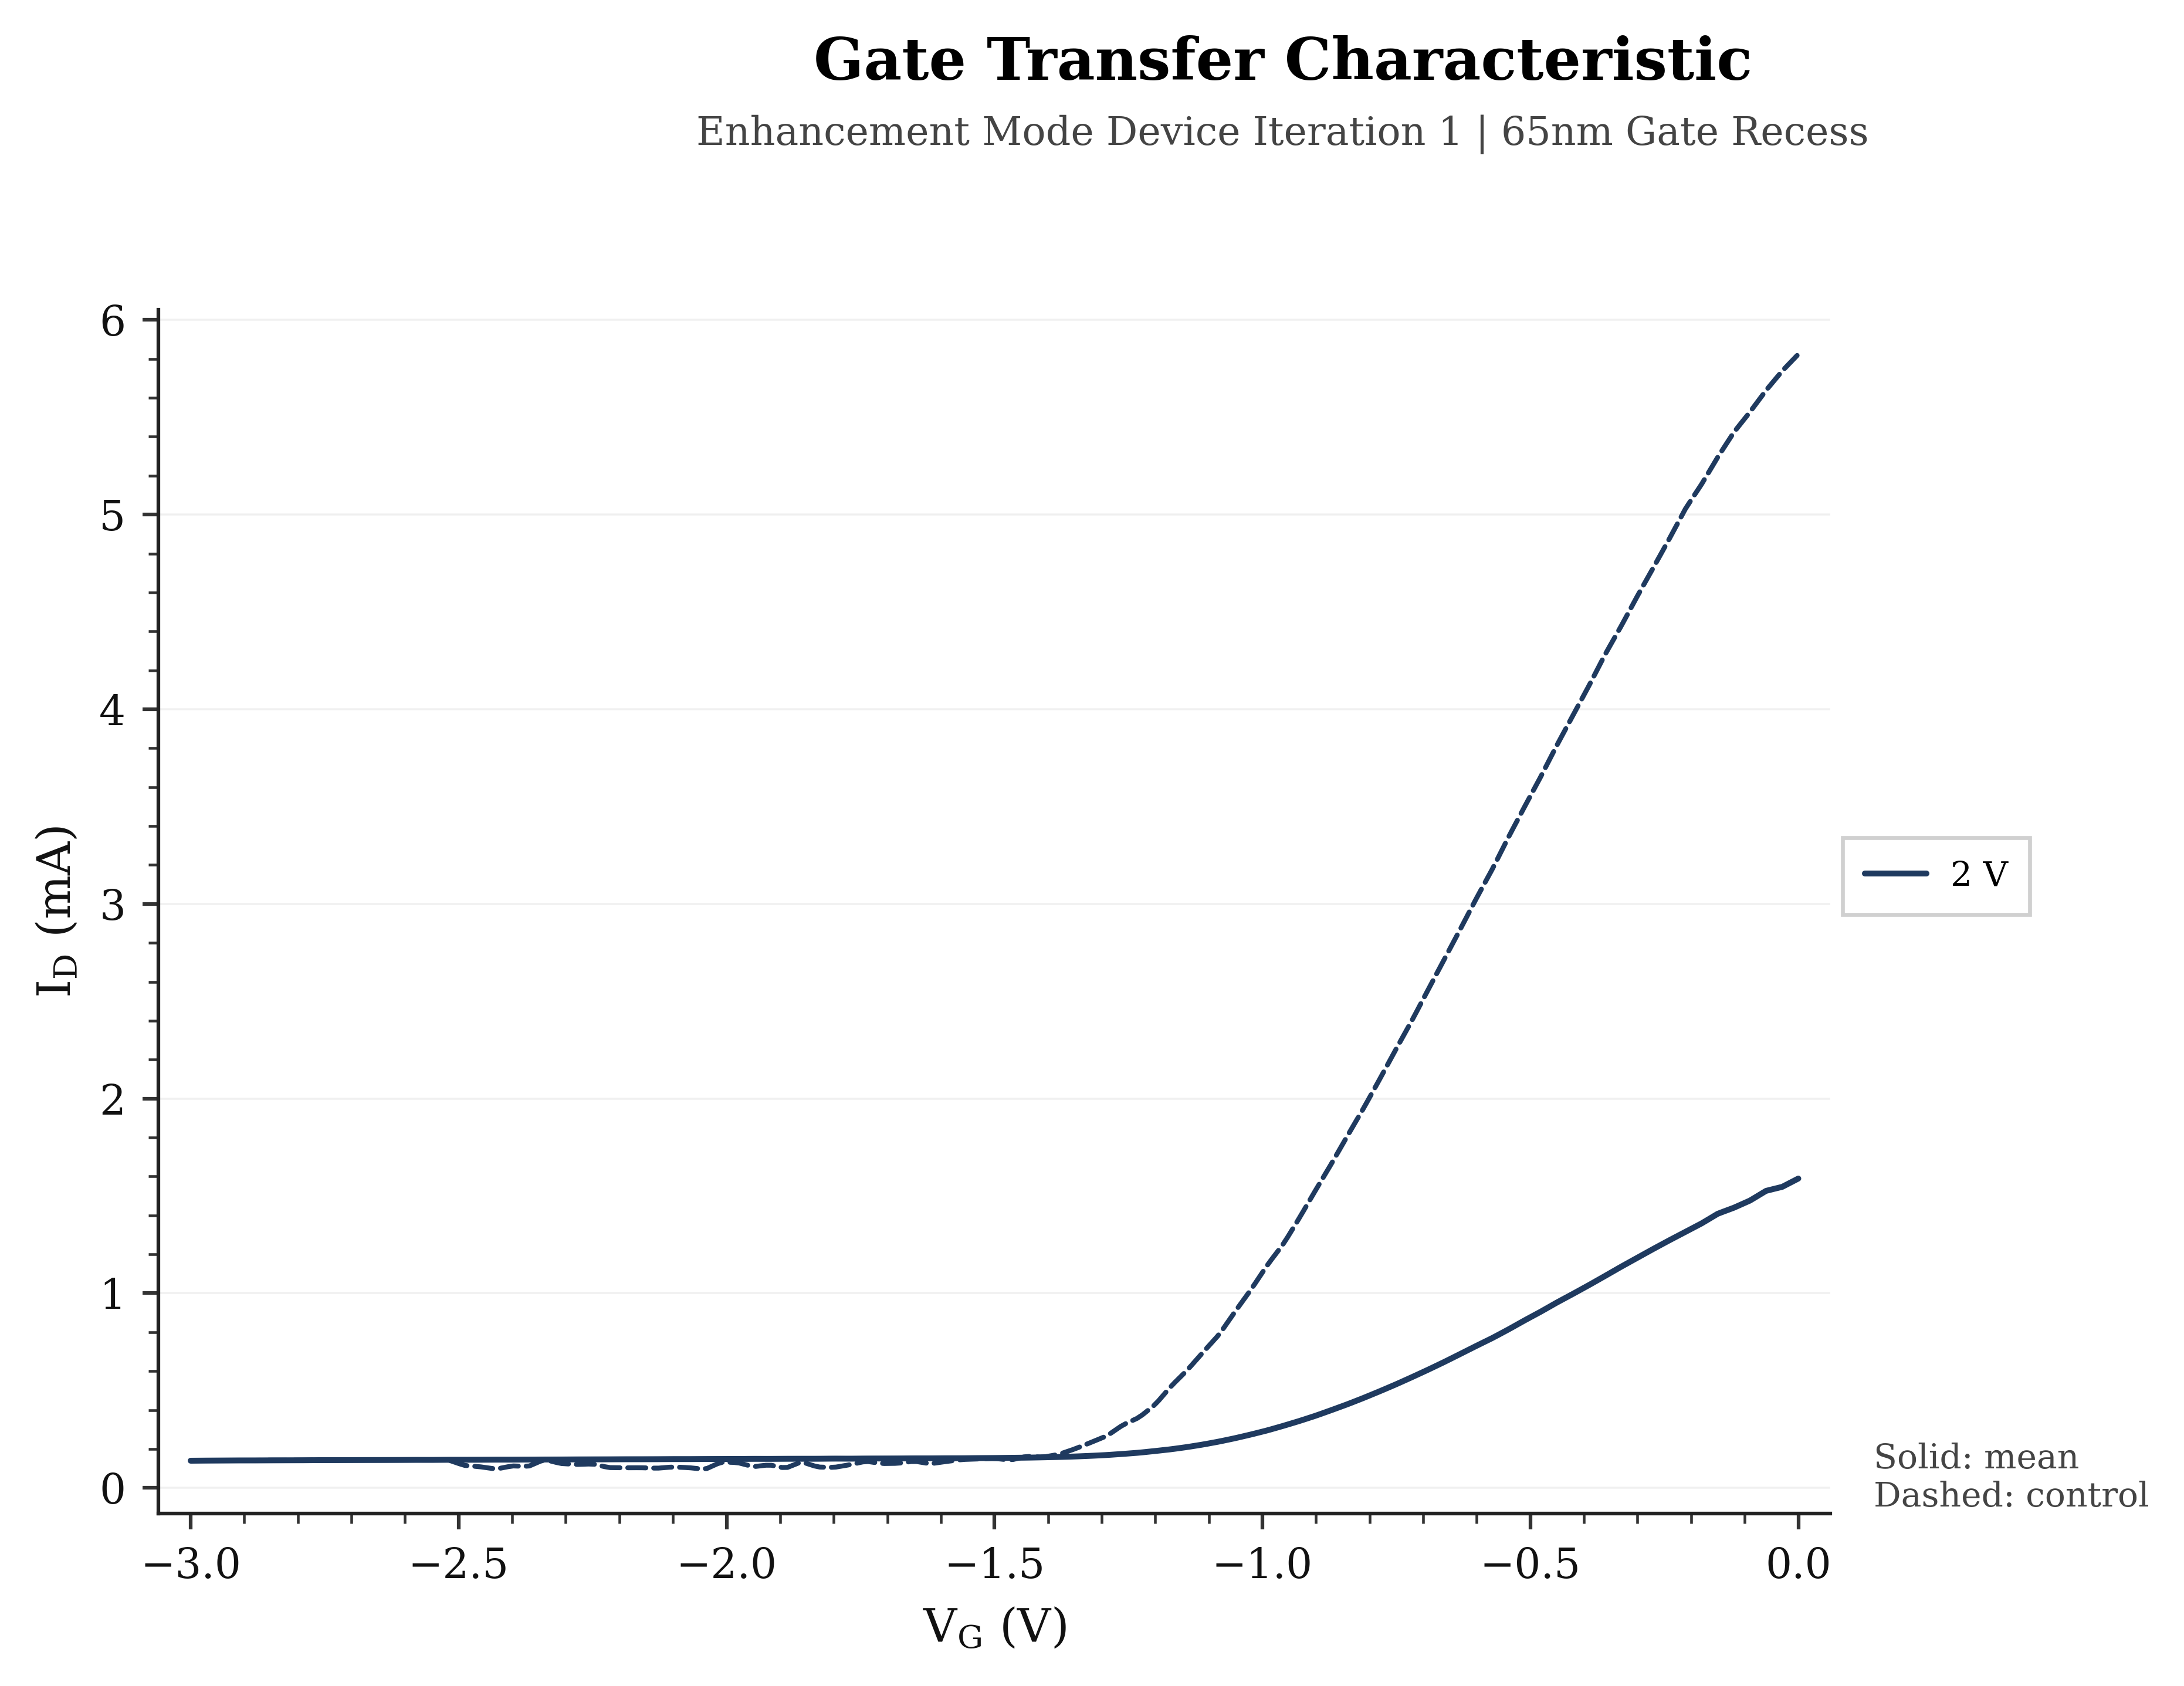
\includegraphics[width=0.9\linewidth]{figures/electrical_analysis/enhancement_mode/iteration_1/65nm_gate_transfer.png}}
  \makebox[\linewidth][c]{\hspace*{-0.04\linewidth}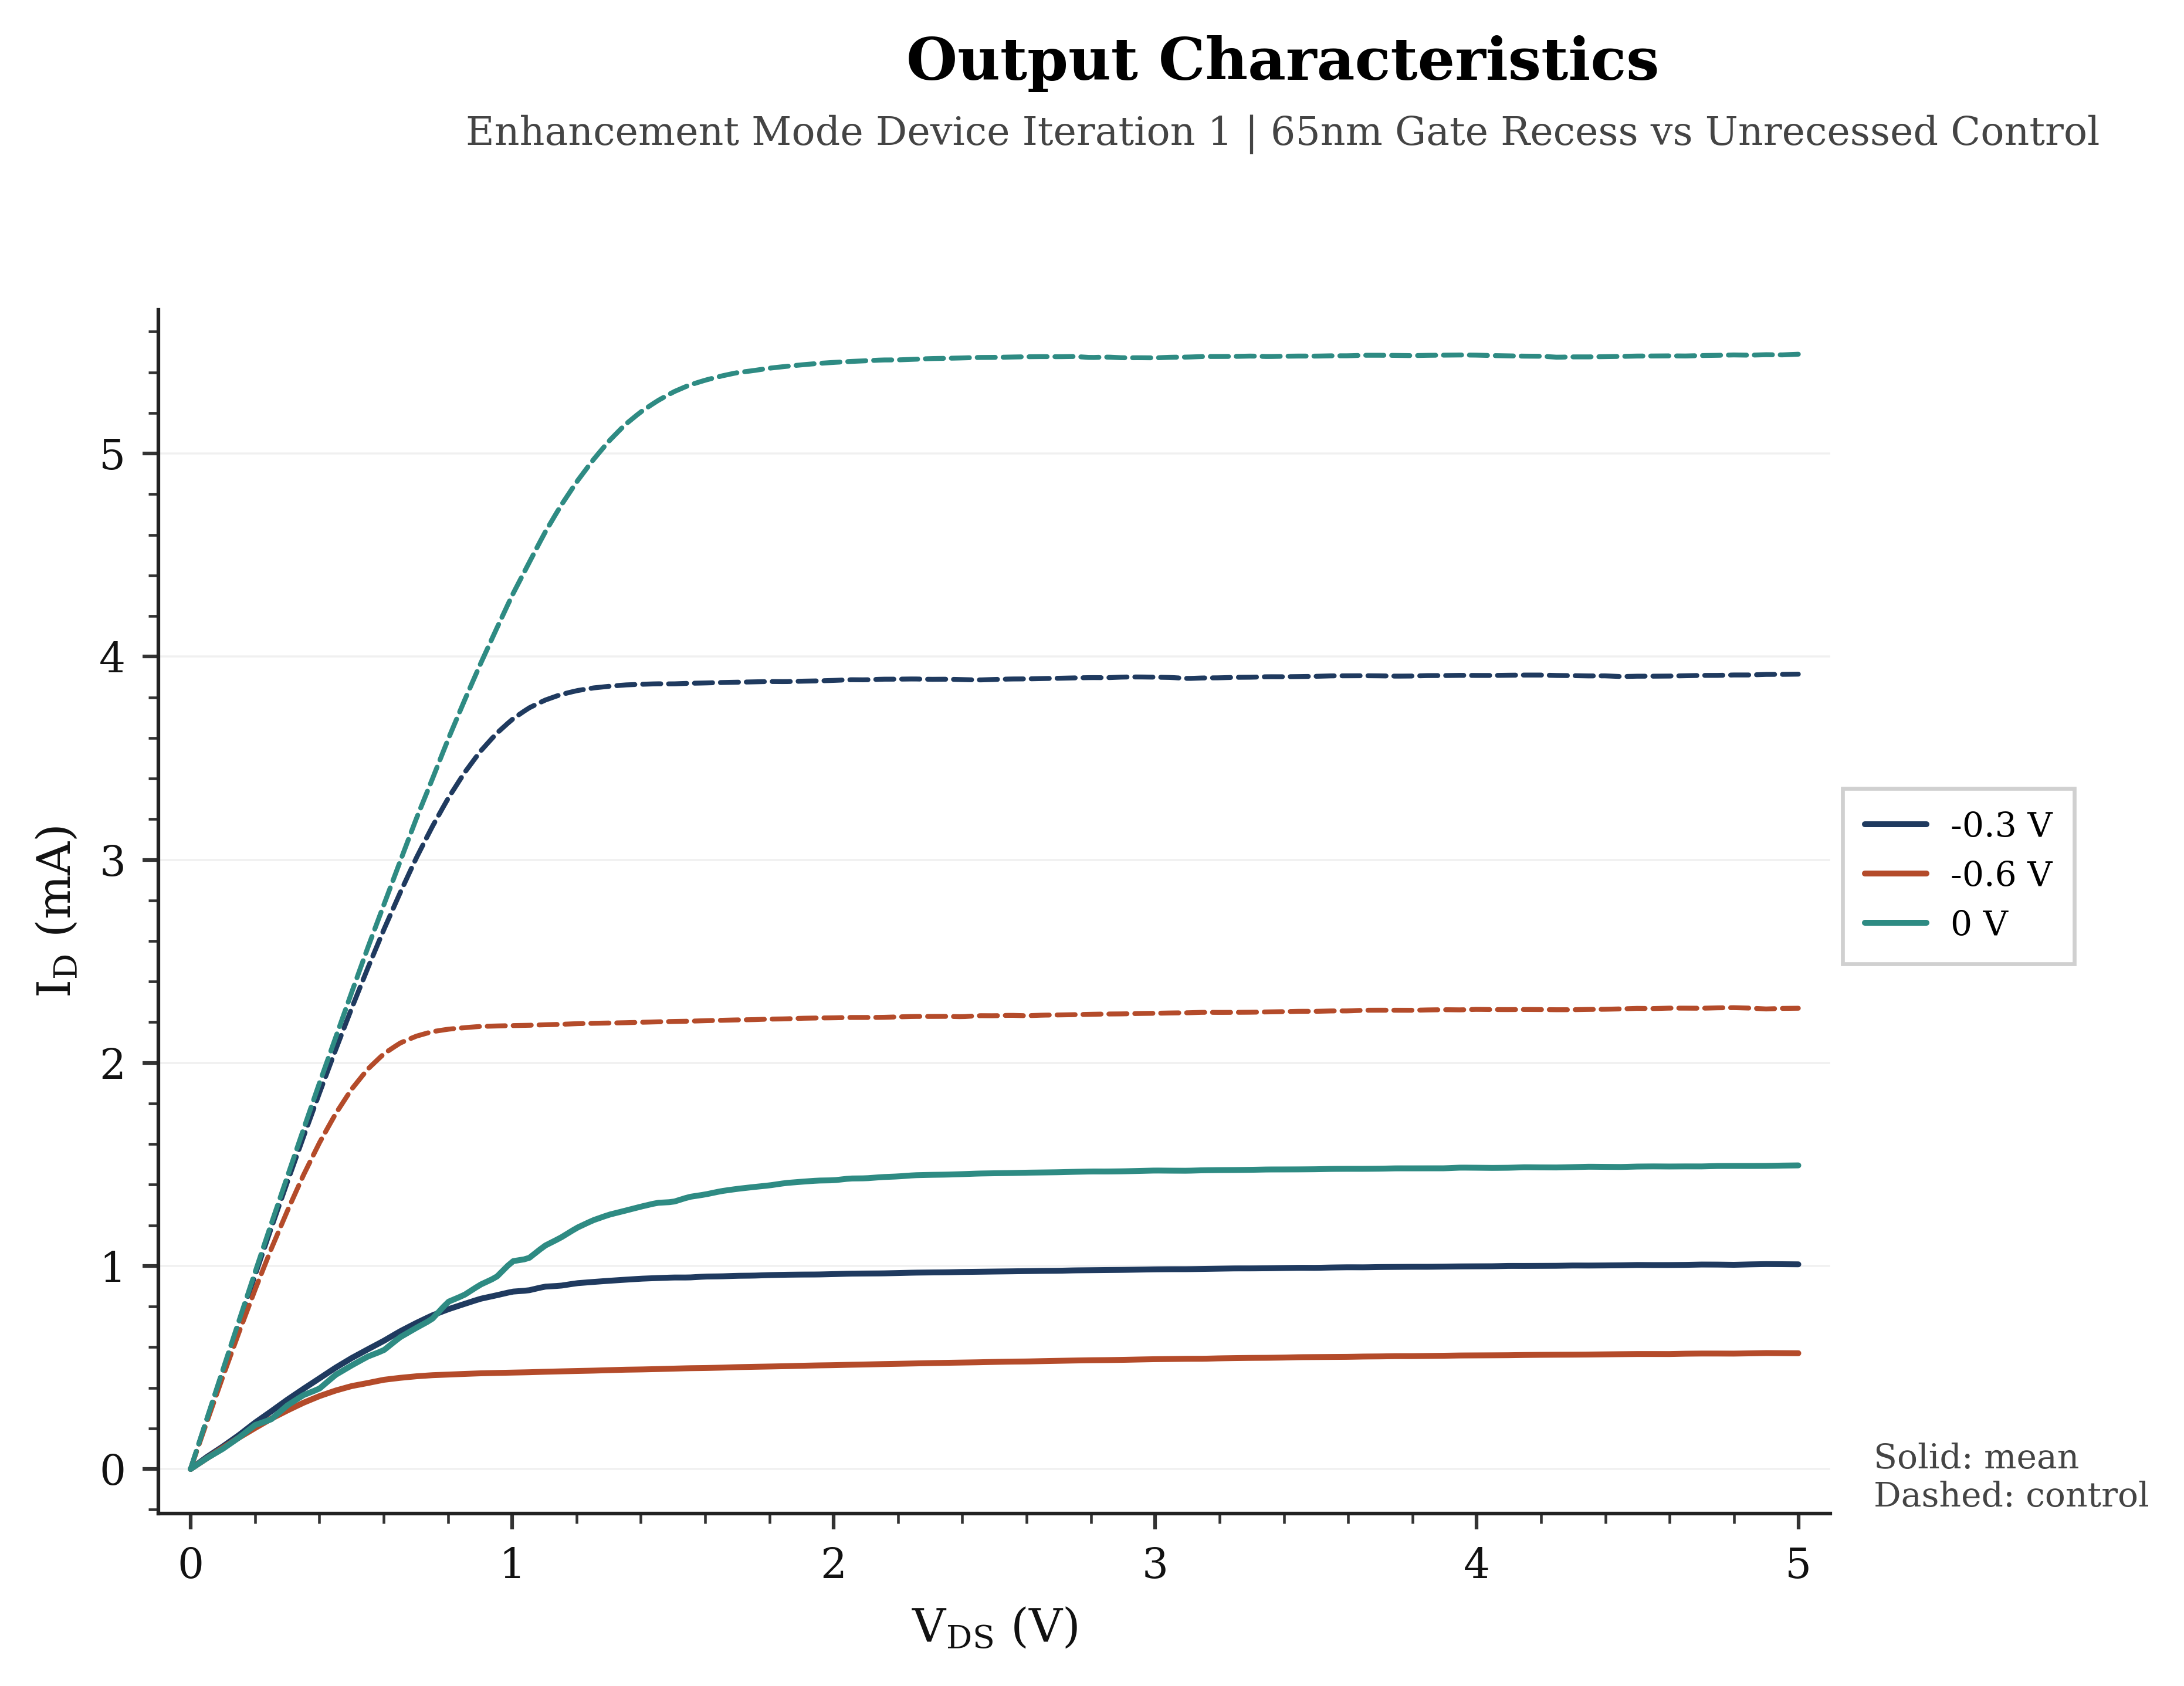
\includegraphics[width=0.9\linewidth]{figures/electrical_analysis/enhancement_mode/iteration_1/65nm_output.png}}
  \vspace{3pt}
  \caption{Iteration 1 electrical comparison between the \SI{65}{\nano\metre}
  recessed device and the unrecessed control device from the same quadrant.}
  \label{fig:iteration1-analysis}
\end{figure}

Figure~\ref{fig:iteration1-analysis} compares the device recessed to
\SI{65}{\nano\metre} with the unrecessed control device from the same
quadrant. The immediate observation is that the recess did not produce the
expected positive shift in threshold voltage. The recessed device still
required negative gate bias to suppress the channel current, so it remained a
depletion-mode device rather than becoming enhancement-mode.

\vspace{1mm}

The main difference introduced by the recess was instead a reduction in drain
current. Across the measured output and transfer characteristics, the
\SI{65}{\nano\metre} recessed device conducted substantially less current than
the unrecessed control. From the gate-transfer curve at
$V_{DS}=\SI{2}{\volt}$, the recessed device reached approximately
\SI{1.6}{\milli\ampere} at $V_G=\SI{0}{\volt}$, compared with approximately
\SI{5.8}{\milli\ampere} for the unrecessed control. This corresponds to a
reduction of roughly \SI{70}{\percent} in the measured drain current at zero
gate bias.

The same trend is visible in the output characteristics. At
$V_{DS}=\SI{5}{\volt}$ and $V_G=\SI{0}{\volt}$, the unrecessed control carried
approximately \SI{5.6}{\milli\ampere}, while the recessed device carried only
approximately \SI{1.5}{\milli\ampere}. At $V_G=\SI{-0.3}{\volt}$, the current
was reduced from approximately \SI{3.9}{\milli\ampere} in the control device
to approximately \SI{1.0}{\milli\ampere} in the recessed device. These
reductions are consistent with removal of donor material from part of the
source--drain path: reducing the available donor charge reduces the carrier
density available for transport, lowering $I_D$ even though the overall
threshold behaviour remains depletion-mode.

\vspace{2mm}
\begin{figure}[htbp]
  \centering
  \makebox[\linewidth][c]{\hspace*{-0.04\linewidth}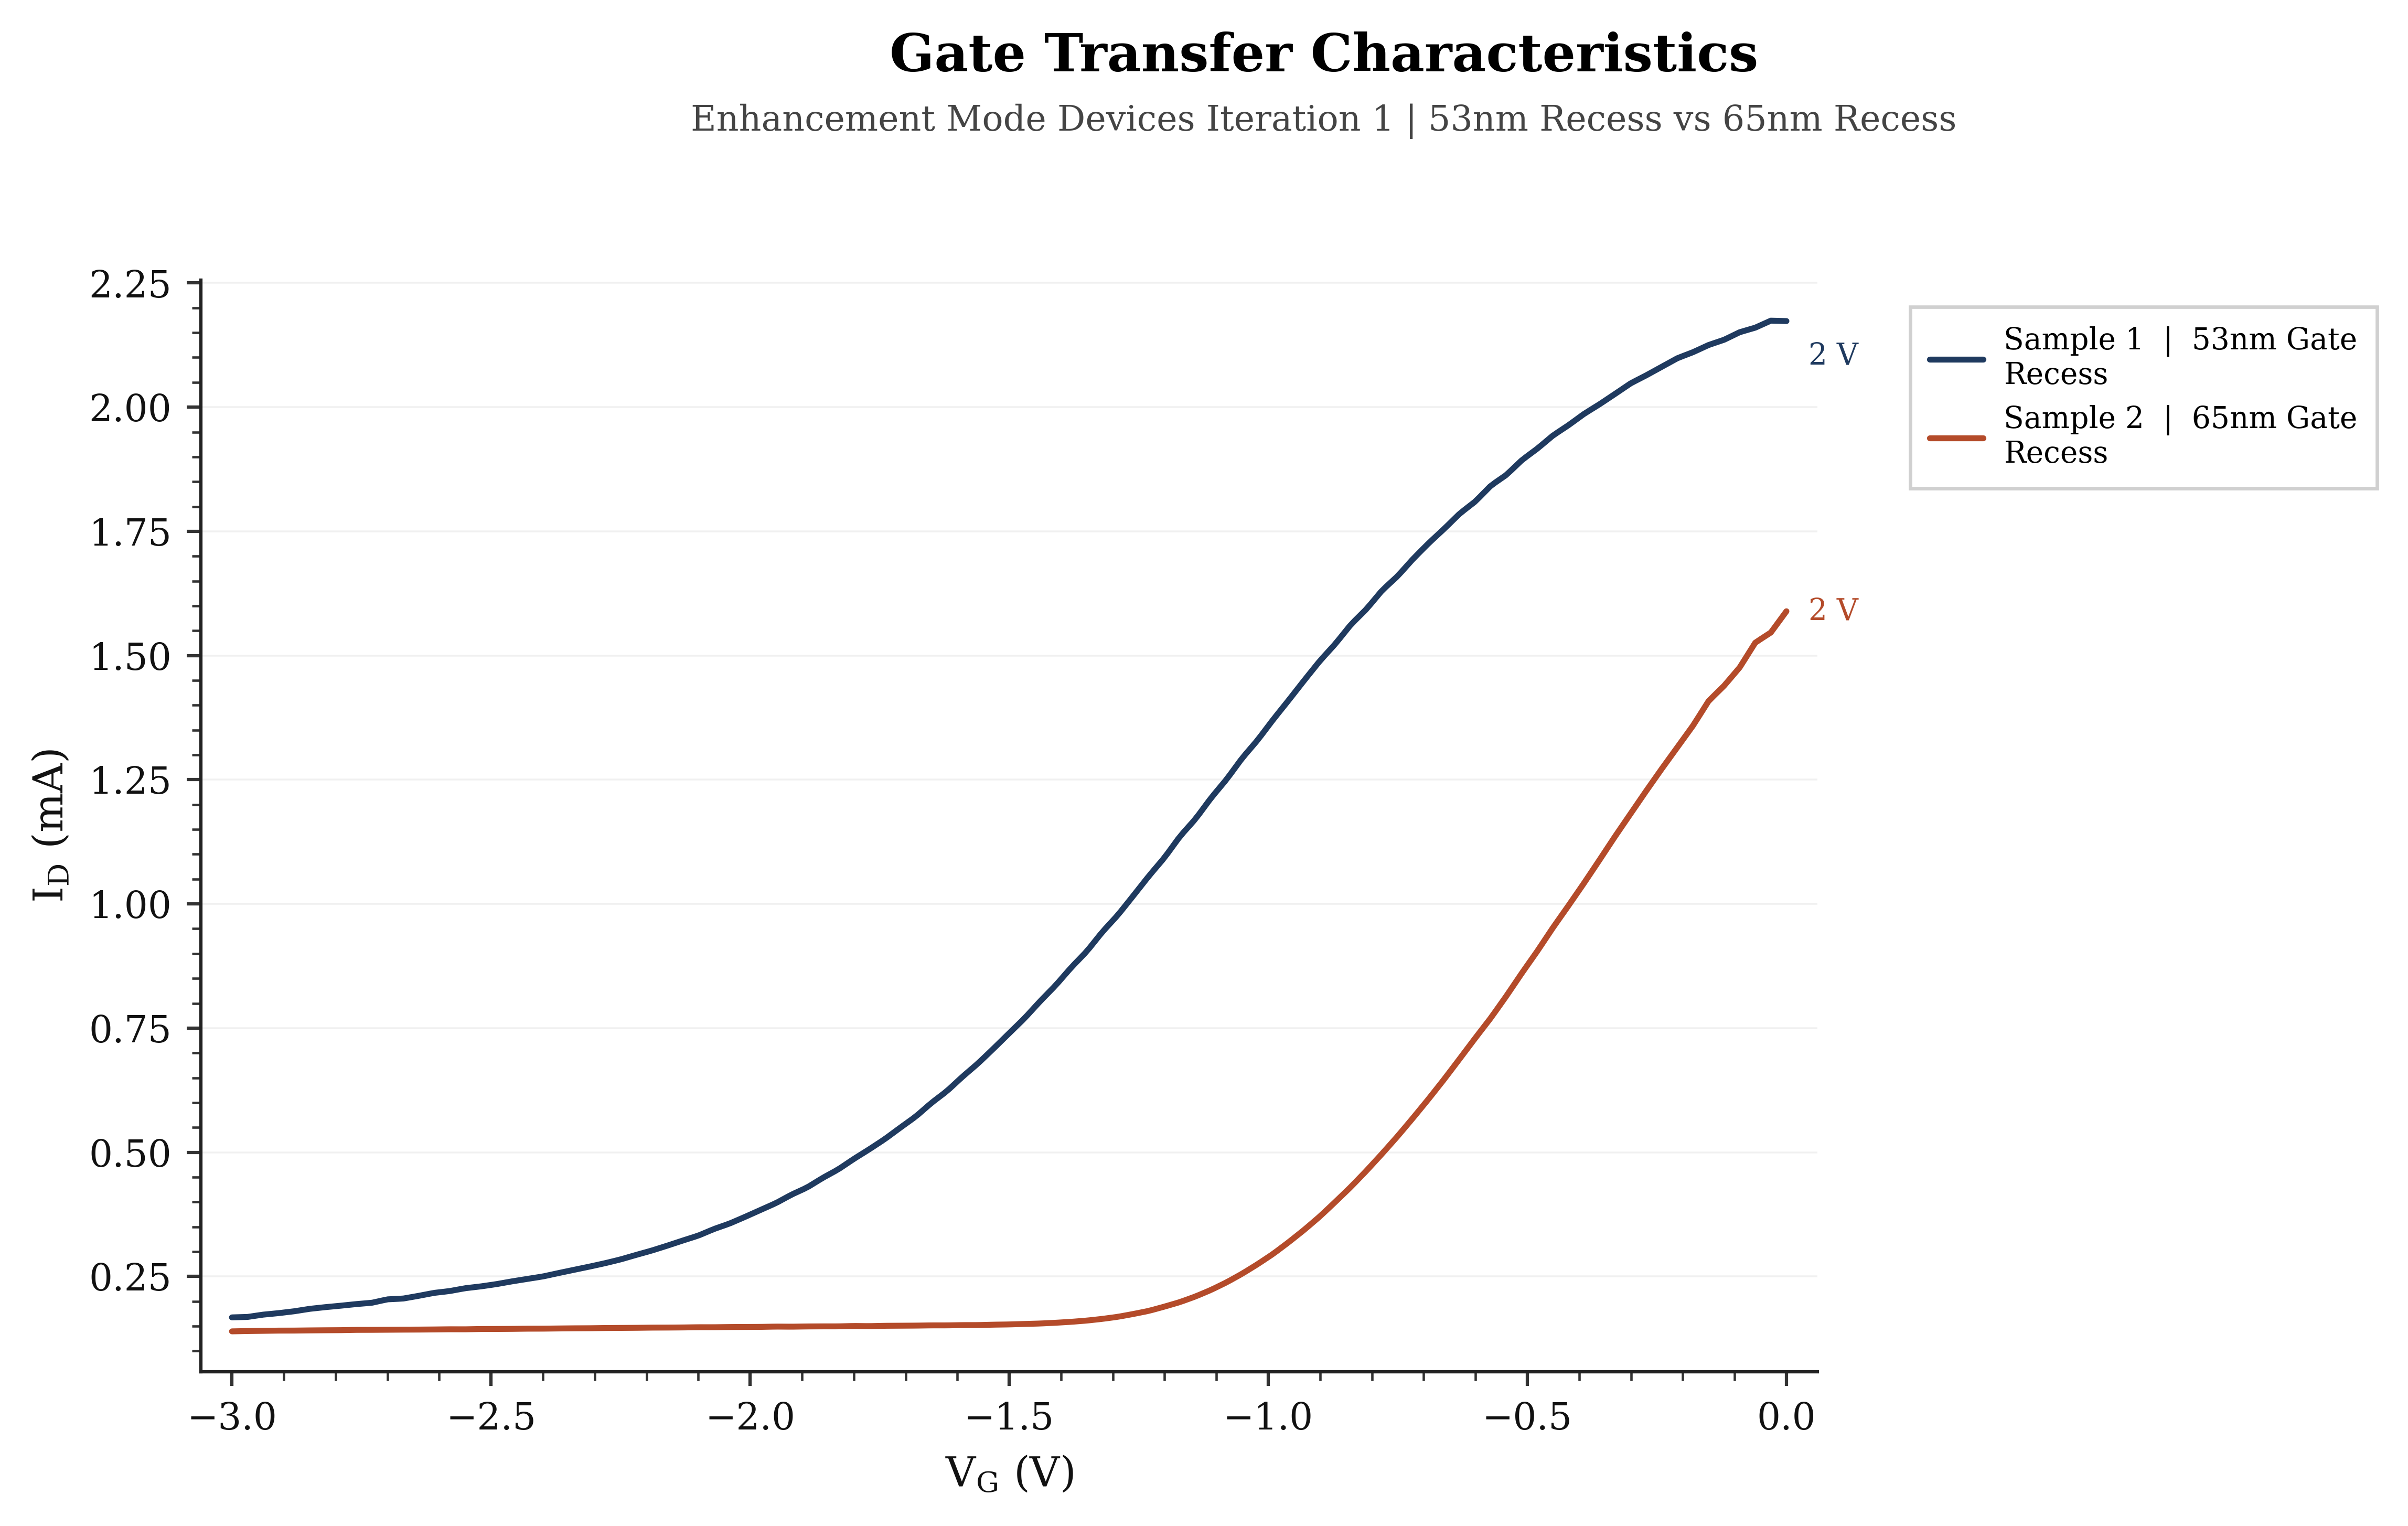
\includegraphics[width=0.9\linewidth]{figures/electrical_analysis/enhancement_mode/iteration_1/53nm_65nm_gate_transfer.png}}
  \caption{Iteration 1 gate-transfer comparison between the
  \SI{53}{\nano\metre} and \SI{65}{\nano\metre} recessed devices.}
  \label{fig:iteration1-analysis-53nm-65nm}
\end{figure}

Figure~\ref{fig:iteration1-analysis-53nm-65nm} investigates this current
reduction further by comparing the two different recessed depths. The
\SI{53}{\nano\metre} recessed device produced higher drain current than the
\SI{65}{\nano\metre} recessed device, indicating that additional material
removal did reduce the conducting charge available in the device. This trend
supports the interpretation that the recess was electrically active and that
the reduced current was not simply a measurement artefact.

At $V_G=\SI{0}{\volt}$ and $V_{DS}=\SI{2}{\volt}$, the
\SI{53}{\nano\metre} recessed device reached approximately
\SI{2.2}{\milli\ampere}, whereas the \SI{65}{\nano\metre} recessed device
reached approximately \SI{1.6}{\milli\ampere}. The shallower recess therefore
carried around \SI{0.6}{\milli\ampere} more current, or approximately
\SI{40}{\percent} more than the deeper recessed device at the same bias point.

However, both recessed devices still showed negative threshold voltages. The
recess depth therefore influenced the magnitude of the drain current, but the
gate was not dominating the device characteristics in the way expected for a
fully recessed source--drain path. The electrical data therefore created a
clear contradiction: the recess was deep enough to reduce current, but not
able to determine the threshold behaviour. This contradiction motivated a
closer examination of the lateral recess geometry.

\FloatBarrier

\section{Iteration Failure Analysis}

Although the excessive recess depth was not the intended process outcome, it
became diagnostically useful. The measured depths suggested that the donor
layer beneath the intended gate region may have been removed too deeply for a
normal channel to remain. If that recessed region had controlled the complete
source--drain path, the devices would be expected to show strongly suppressed
conduction or fail to operate. Instead, functioning depletion-mode HEMTs were
measured. This made clear that the current gate-recess geometry was not able
to fully dominate the electrical characteristics of the device.

The primary failure mechanism was therefore the lateral geometry of the recess
itself. Although the recess slits were positioned between source and drain,
they did not span the full active conduction region controlled by the gate. The
original GaAs/AlGaAs heterostructure was therefore left intact in adjacent
regions, allowing a 2DEG to form at zero gate bias and current to flow around
the locally recessed trench.

This current-spreading mechanism is illustrated in
Figure~\ref{fig:iteration-1-current-bypass}, where the red arrows show
possible lateral paths around the corners of the locally recessed trench.

% ------------------------------------------------------------
% File: figures/fig-current-path-bypass.tex
% Iteration 1 bypass current path annotation
% ------------------------------------------------------------

\begin{figure}[htbp]
  \centering
  \begin{tikzpicture}[
    font=\footnotesize,
    imglabel/.style={draw, fill=white, line width=0.35pt, inner xsep=4pt,
      inner ysep=2pt, font=\small\bfseries},
    recessbox/.style={dashed, line width=2.2pt},
    current/.style={-Latex, line width=2.5pt, rounded corners=8pt},
    blocked/.style={dashed, line width=0.9pt, opacity=0.70}
  ]
    \node[anchor=north west, inner sep=0pt] (device) at (0,0) {
      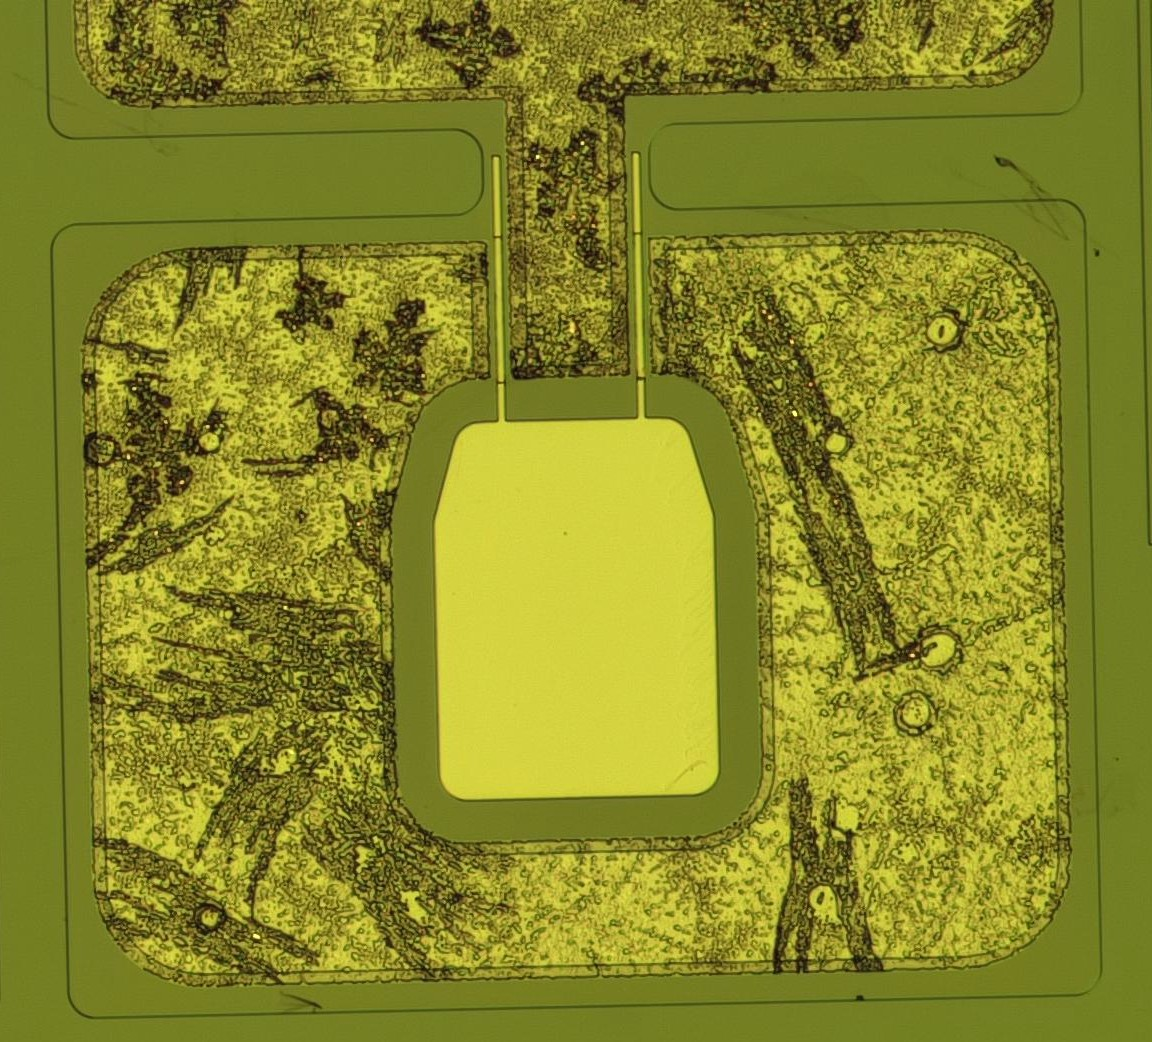
\includegraphics[width=0.70\linewidth]{figures/fabrication_images/enhancement_mode_images/current_path_annotate.jpg}
    };

    % Manual adjustment controls. Fractions are measured from the top-left of
    % the microscopy image. Reduce/increase the vertical height of the blue
    % recess box by changing \recessBoxTop and \recessBoxBottom.
    \def\recessBoxLeft{0.41}
    \def\recessBoxRight{0.57}
    \def\recessBoxTop{0.25}
    \def\recessBoxBottom{0.360}

    % Coordinates are fractional positions measured from the top-left of the
    % microscopy image. Adjust these values if the annotation needs fine tuning.
    \path let \p1=(device.north west), \p2=(device.south east) in
      coordinate (sourceLabel) at ({\x1+0.50*(\x2-\x1)}, {\y1+0.86*(\y2-\y1)})
      coordinate (drainLabel) at ({\x1+0.50*(\x2-\x1)}, {\y1+0.18*(\y2-\y1)})
      coordinate (gateLabel) at ({\x1+0.50*(\x2-\x1)}, {\y1+0.60*(\y2-\y1)})
      coordinate (recessNW) at ({\x1+\recessBoxLeft*(\x2-\x1)}, {\y1+\recessBoxTop*(\y2-\y1)})
      coordinate (recessSE) at ({\x1+\recessBoxRight*(\x2-\x1)}, {\y1+\recessBoxBottom*(\y2-\y1)})
      coordinate (leftUpperStart) at ({\x1+0.305*(\x2-\x1)}, {\y1+0.275*(\y2-\y1)})
      coordinate (leftUpperA) at ({\x1+0.382*(\x2-\x1)}, {\y1+0.200*(\y2-\y1)})
      coordinate (leftUpperB) at ({\x1+0.412*(\x2-\x1)}, {\y1+0.198*(\y2-\y1)})
      coordinate (leftUpperEnd) at ({\x1+0.487*(\x2-\x1)}, {\y1+0.266*(\y2-\y1)})
      coordinate (leftLowerStart) at ({\x1+0.305*(\x2-\x1)}, {\y1+0.380*(\y2-\y1)})
      coordinate (leftLowerA) at ({\x1+0.375*(\x2-\x1)}, {\y1+0.435*(\y2-\y1)})
      coordinate (leftLowerEnd) at ({\x1+0.490*(\x2-\x1)}, {\y1+0.362*(\y2-\y1)})
      coordinate (rightUpperStart) at ({\x1+0.695*(\x2-\x1)}, {\y1+0.275*(\y2-\y1)})
      coordinate (rightUpperA) at ({\x1+0.598*(\x2-\x1)}, {\y1+0.200*(\y2-\y1)})
      coordinate (rightUpperB) at ({\x1+0.568*(\x2-\x1)}, {\y1+0.198*(\y2-\y1)})
      coordinate (rightUpperEnd) at ({\x1+0.513*(\x2-\x1)}, {\y1+0.266*(\y2-\y1)})
      coordinate (rightLowerStart) at ({\x1+0.695*(\x2-\x1)}, {\y1+0.380*(\y2-\y1)})
      coordinate (rightLowerA) at ({\x1+0.605*(\x2-\x1)}, {\y1+0.435*(\y2-\y1)})
      coordinate (rightLowerEnd) at ({\x1+0.510*(\x2-\x1)}, {\y1+0.362*(\y2-\y1)})
      coordinate (recessText) at ({\x1+0.49*(\x2-\x1)}, {\y1+0.305*(\y2-\y1)});

    \draw[recessbox, white, opacity=0.85] (recessNW) rectangle (recessSE);
    \draw[recessbox, blue!90!black] (recessNW) rectangle (recessSE);

    \node[imglabel, font=\footnotesize\bfseries, align=center]
      at (recessText) {local recessed trenches};

    \draw[current, red!80!black]
      (leftUpperStart) -- (leftUpperA) -- (leftUpperB) -- (leftUpperEnd);
    \draw[current, red!80!black]
      (leftLowerStart) -- (leftLowerA) -- (leftLowerEnd);
    \draw[current, red!80!black]
      (rightUpperStart) -- (rightUpperA) -- (rightUpperB) -- (rightUpperEnd);
    \draw[current, red!80!black]
      (rightLowerStart) -- (rightLowerA) -- (rightLowerEnd);

    \node[imglabel] at (sourceLabel) {Source};
    \node[imglabel] at (drainLabel) {Drain};
    \node[imglabel] at (gateLabel) {Gate};
  \end{tikzpicture}

  \vspace{2mm}
  \caption{Annotated microscopy image showing how current can bypass the local
  recessed trench through adjacent unrecessed regions between source and drain.
  The red arrows indicate possible lateral source--drain current paths passing
  around the upper and lower corners of the recessed region.}
  \label{fig:iteration-1-current-bypass}
\end{figure}


This bypass path explains why the devices remained depletion-mode despite the
large measured recess depths. The extracted threshold voltage reflects the
combined response of the recessed and unrecessed geometry, rather than the
threshold of a uniformly recessed channel. For this reason, the Iteration 1 data
cannot be used to extract a reliable relationship between recess depth and
threshold voltage.

\section{Iteration Conclusion}

Iteration 1 demonstrated that the basic fabrication sequence for recessed-gate
devices was feasible and could be completed. The samples were successfully processed through
the shared mesa and ohmic-contact stages, the quadrant-specific recess and
gate steps were carried out, and the gate metal was optically confirmed to
cover the etched trenches as designed.

However, the iteration also revealed the central limitation of this first
design: local trench recession was insufficient unless the measured
source--drain current was forced to pass through the recessed region. The
over-etched devices were surprisingly useful because they exposed this geometry
problem directly. 
